\documentclass[aspectratio=169]{beamer}
\usetheme{metropolis}
\setbeamertemplate{frame footer}{
\includegraphics[height=0.25cm]{figs/UC_Santa_Barbara}}
\usepackage{graphicx}
\usepackage{subcaption}
\usepackage{amsmath}
\usepackage{amssymb}

% Title information
\title[Neural Population Geometry]{Neural Population Geometry}
\subtitle{ME 225NN, Winter 2025}
\author[Acosta \& Skaza]{Santiago Acosta \& Jonathan Skaza}
\institute[UCSB]{Dynamical Neuroscience Graduate Program\\University of California, Santa Barbara}
\date{}

\begin{document}

% Title slide
\begin{frame}
    \titlepage
\end{frame}

% Outline slide
\begin{frame}{Outline}
    \tableofcontents
\end{frame}

% Introduction section
\section{Introduction}

\begin{frame}{Problem Description \& Motivation}
    \begin{itemize}
        \item Advances in recording techniques: thousands to millions of neurons simultaneously
        \item Challenges in studying large neural populations:
        \begin{itemize}
            \item Neurons respond to multiple variables simultaneously
            \item Traditional tuning-based analyses have limitations for complex tasks
        \end{itemize}
        \item Shift from single-neuron tuning to \textit{geometric} approaches
        \item Neural computations emerge from structured, high-dimensional activity patterns
        \item Neural manifolds: low-dimensional geometric structures in high-dimensional neural state space
    \end{itemize}
\end{frame}

\begin{frame}{Neural Manifolds}
    \begin{itemize}
        \item Key properties of neural manifolds:
        \begin{itemize}
            \item Dimensionality: intrinsic dimensions of the representation
            \item Curvature: how the manifold deviates from flat space
            \item Separability: distinguishability between different manifolds
            \item Capacity: number of distinct manifolds a system can support
        \end{itemize}
        \item Examples of manifold structures in the brain:
        \begin{itemize}
            \item Ring-shaped manifolds in hippocampus (head direction)
            \item Ring-shaped manifolds in visual cortex (orientation)
        \end{itemize}
        \item Direct mappings between manifold geometry and task variables provide mechanistic insights
    \end{itemize}
\end{frame}

\begin{frame}{Bridging Biological and Artificial Neural Networks}
    \begin{itemize}
        \item Neural population geometry provides a unified framework for understanding:
        \begin{itemize}
            \item Biological neural circuits
            \item Artificial neural networks (ANNs)
        \end{itemize}
        \item Neural computation as geometric transformations
        \item Population-level representations enable:
        \begin{itemize}
            \item Robust information processing
            \item Efficient encoding
            \item Scalable computation
        \end{itemize}
        \item Reveals fundamental principles that transcend specific implementations
    \end{itemize}
\end{frame}

\begin{frame}{Paper Summary}
    \begin{itemize}
        \item We demonstrate neural population geometry as a unified framework for understanding information encoding
        \item Focus on representation of circular variables—a fundamental computational challenge
        \item Parallel analyses of:
        \begin{itemize}
            \item Orientation encoding in mouse visual cortex
            \item Trained convolutional neural network (CNN)
        \end{itemize}
        \item Show how similar ring-shaped manifolds emerge in both systems
        \item Circular manifolds arise from computational demands rather than architectural constraints
        \item Comparative approach reveals common principles across biological and artificial systems
    \end{itemize}
\end{frame}

% Preliminaries section
\section{Preliminaries}

\begin{frame}{Neural State Space \& Population Activity}
    \begin{columns}
        \column{0.5\textwidth}
        \begin{itemize}
            \item Neural state space: each axis represents a single neuron
            \item Population activity: $\mathbf{r} = (r_1, r_2, \ldots, r_n) \in \mathbb{R}^n$
            \item Repeated stimulus presentations create point clouds
            \item Neural variability induces fluctuations
            \item Manifolds emerge from stimulus responses
        \end{itemize}
        
        \column{0.5\textwidth}
        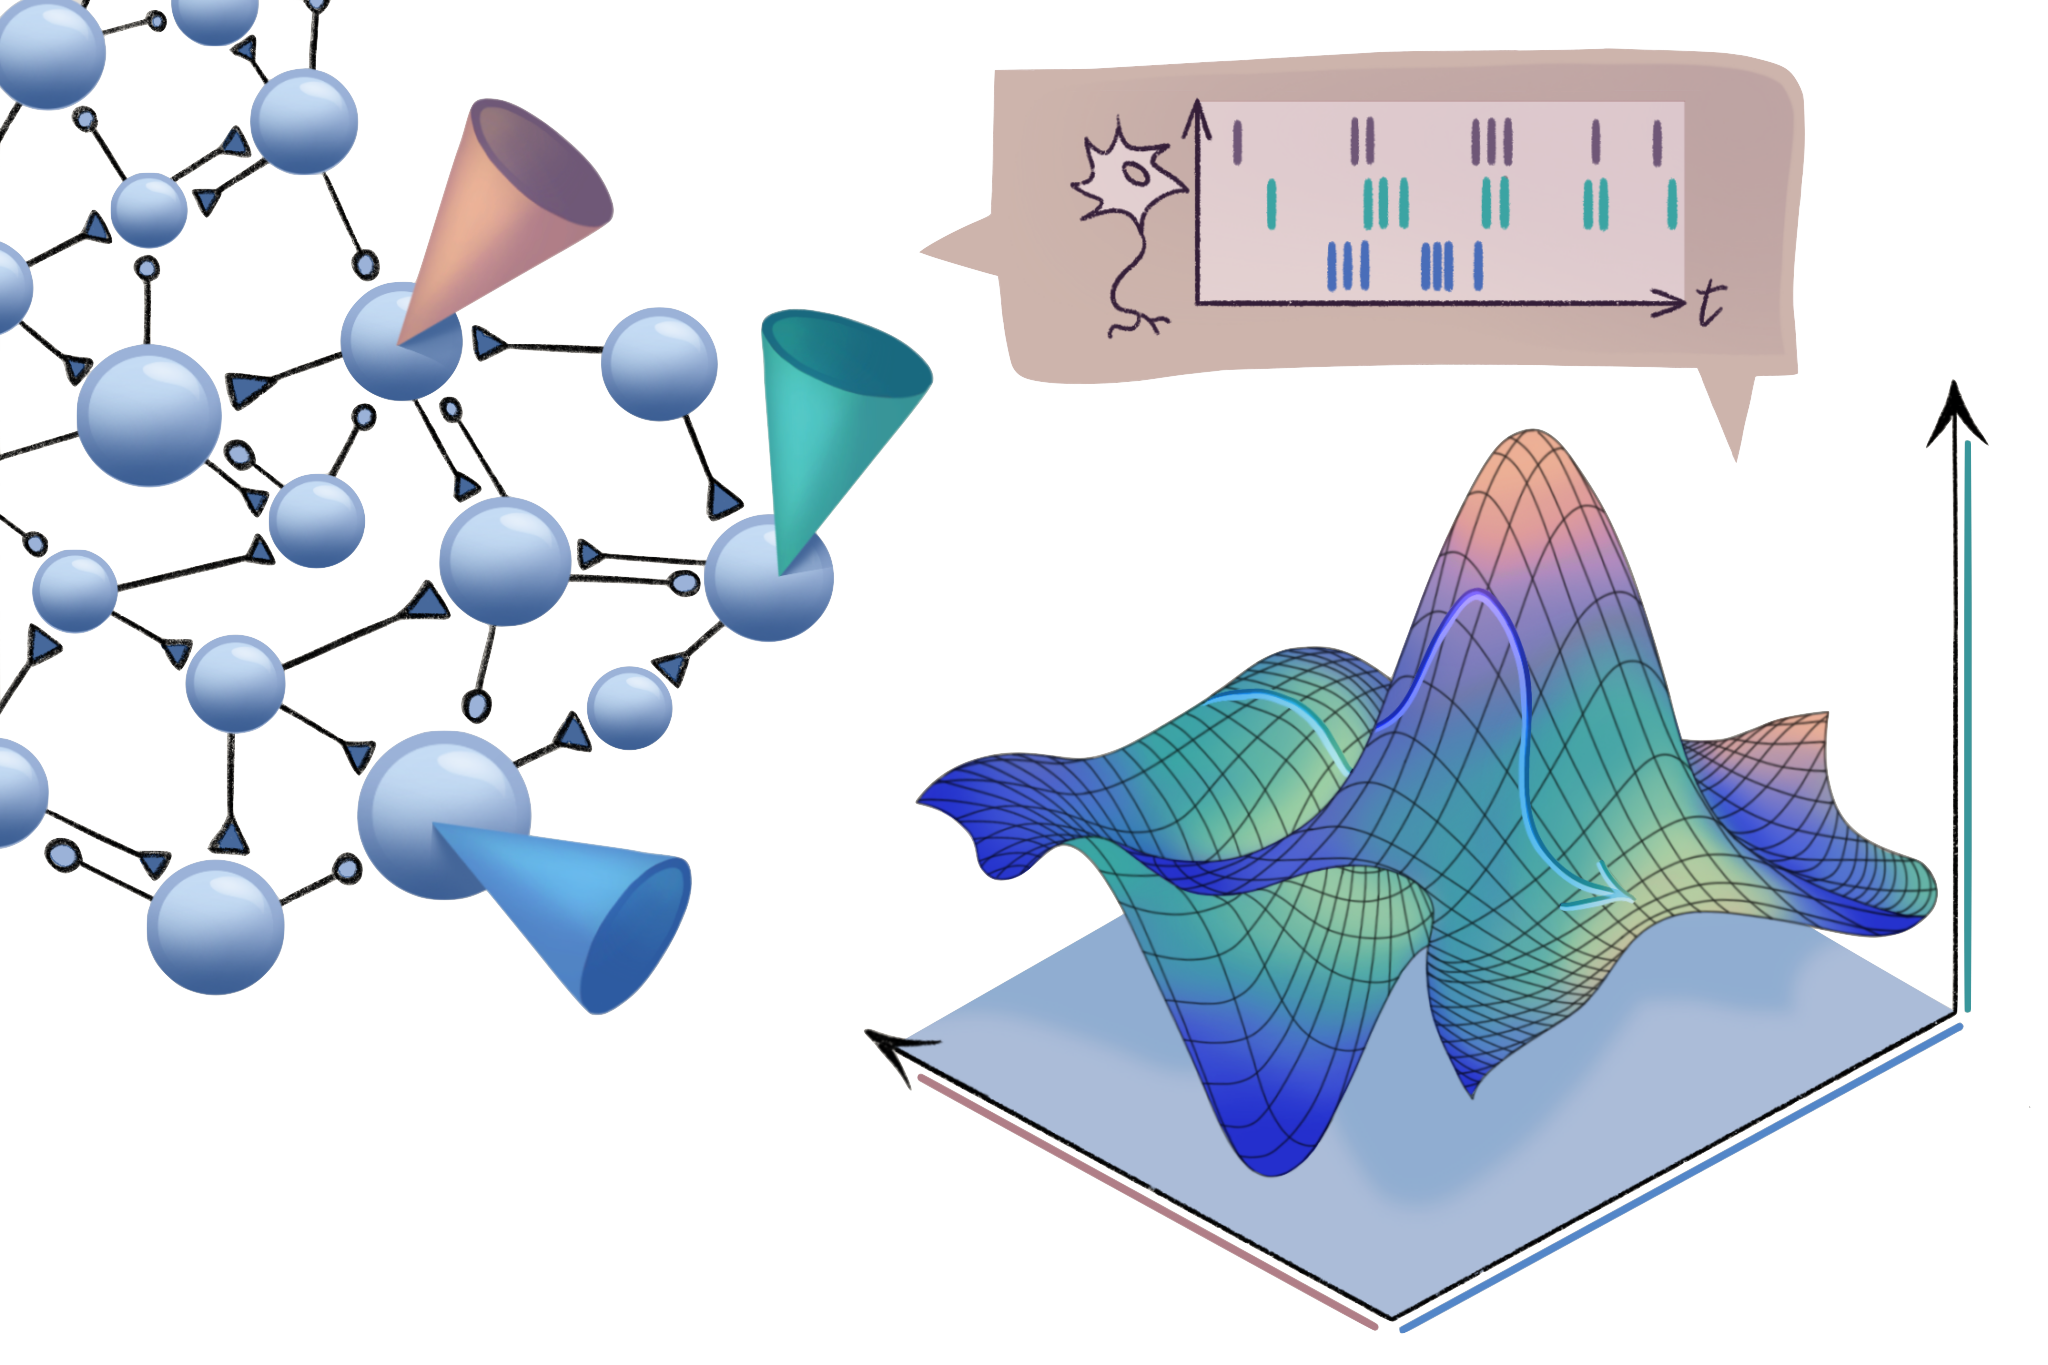
\includegraphics[width=\textwidth]{figs/manifold_schematic.png}
    \end{columns}
\end{frame}

\begin{frame}{Mathematical Foundations of Neural Manifolds}
    \begin{itemize}
        \item \textbf{Manifold}: Topological space that locally resembles Euclidean space
        \item \textbf{Neural manifold}: Population activity constrained to lower-dimensional subspace
        \item Formal definition: For stimulus condition $s$, the neural manifold $\mathcal{M}_s$ is:
        \begin{equation}
        \mathcal{M}_s = \{\mathbf{r}(t) \in \mathbb{R}^n : \text{condition } s \text{ is presented at time } t\}
        \end{equation}
        \item Real neural data extends beyond strict mathematical definition:
        \begin{itemize}
            \item Neural variability creates point clouds rather than isolated points
            \item Experimental limitations lead to sparse sampling of the manifold
        \end{itemize}
    \end{itemize}
\end{frame}

\begin{frame}{Types of Neural Manifolds}
    \begin{itemize}
        \item \textbf{Object/perceptual manifolds}: Arise from identity-preserving variations
        \begin{equation}
        \mathcal{M}_{\text{obj}} = \{f(T_\theta(\mathbf{x})) : \theta \in \Theta\}
        \end{equation}
        where $f$ is neural encoding function, $T_\theta$ is transformation with parameter $\theta$
        
        \item \textbf{Point-cloud manifolds}: Empirical manifestation in experimental data
        \begin{equation}
        \hat{\mathcal{M}} = \{\mathbf{r}_i : i = 1, 2, \ldots, k\}
        \end{equation}
        for stimuli $\{s_1, s_2, \ldots, s_k\}$ and responses $\{\mathbf{r}_1, \mathbf{r}_2, \ldots, \mathbf{r}_k\}$
    \end{itemize}
\end{frame}

\begin{frame}{Manifold Estimation Techniques}
    \begin{itemize}
        \item \textbf{Linear dimensionality reduction}:
        \begin{itemize}
            \item Principal Component Analysis (PCA)
            \item Efficient but misses nonlinear structure
        \end{itemize}
        
        \item \textbf{Nonlinear dimensionality reduction}:
        \begin{itemize}
            \item Isomap, t-SNE, MDS, UMAP, etc.
            \item Preserve geometric relationships
            \item May fail with complex topological structures
        \end{itemize}
        
        \item \textbf{Topologically-motivated methods}:
        \begin{itemize}
            \item SPUD (Spline Parameterization for Unsupervised Decoding)
            \item Persistent homology
            \item Essential for circular or toroidal structures
        \end{itemize}
    \end{itemize}
\end{frame}

% Neural Population Geometry section
\section{Neural Population Geometry}

\begin{frame}{Key Concepts in Neural Population Geometry}
    \begin{itemize}
        \item \textbf{Dimensionality}: Intrinsic dimensionality $d$ of manifold $\mathcal{M}$
        \begin{itemize}
            \item Estimated using PCA or nonlinear methods
        \end{itemize}
        
        \item \textbf{Curvature}: How manifold deviates from flat space
        \begin{itemize}
            \item High curvature: small stimulus changes → large neural response changes
        \end{itemize}
        
        \item \textbf{Separability}: Distinguishability between manifolds
        \begin{equation}
        d(\mathcal{M}_i, \mathcal{M}_j) = \min_{\mathbf{r}_i \in \mathcal{M}_i, \mathbf{r}_j \in \mathcal{M}_j} \|\mathbf{r}_i - \mathbf{r}_j\|
        \end{equation}
        
        \item \textbf{Capacity}: Number of distinct manifolds a neural system can support
    \end{itemize}
\end{frame}

% Simulation section
\section{Simulation Study}

\begin{frame}{Circular Variables Experiment}
    \begin{itemize}
        \item Demonstration of geometric structures in neural representations
        \item Simulation experiment: encoding circular variables
        \item Illustrates how topological structures naturally emerge
        \item CNN trained to predict orientation of visual grating stimuli
        \item Analogous to orientation selectivity in visual cortex
    \end{itemize}
    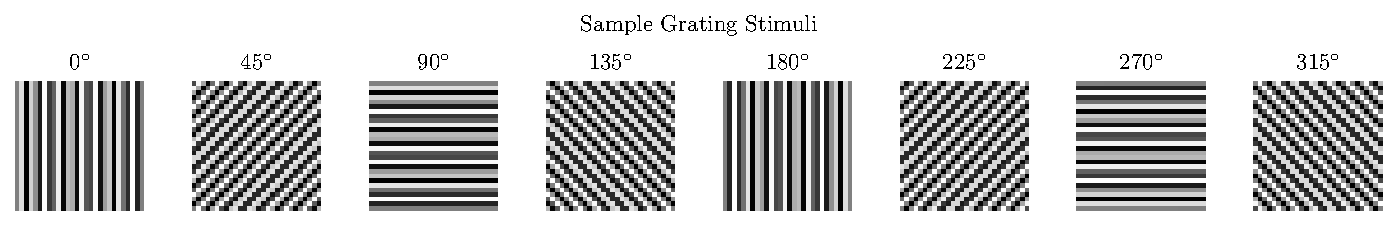
\includegraphics[width=0.7\textwidth]{results/grating_samples.pdf}
    \captionof{figure}{Sample grating stimuli at different orientations}
\end{frame}

\begin{frame}{CNN Architecture}
    \begin{itemize}
        \item Convolutional layers followed by fully connected layers
        \item 32-dimensional latent space analyzed for geometric properties
        \item Network trained to predict sine and cosine components of orientation angle
        \item Sine-cosine encoding naturally handles circular topology
        \begin{itemize}
            \item For small $\epsilon$, angles $\epsilon$ and $2\pi - \epsilon$ are similar orientations
            \item But numerically distant in raw angle representation
            \item With sine-cosine: $(\cos(\epsilon), \sin(\epsilon)) \approx (\cos(2\pi-\epsilon), \sin(2\pi - \epsilon)) \approx (1, 0)$
        \end{itemize}
    \end{itemize}
\end{frame}

\begin{frame}{Results: Circular Manifold}
    \centering
    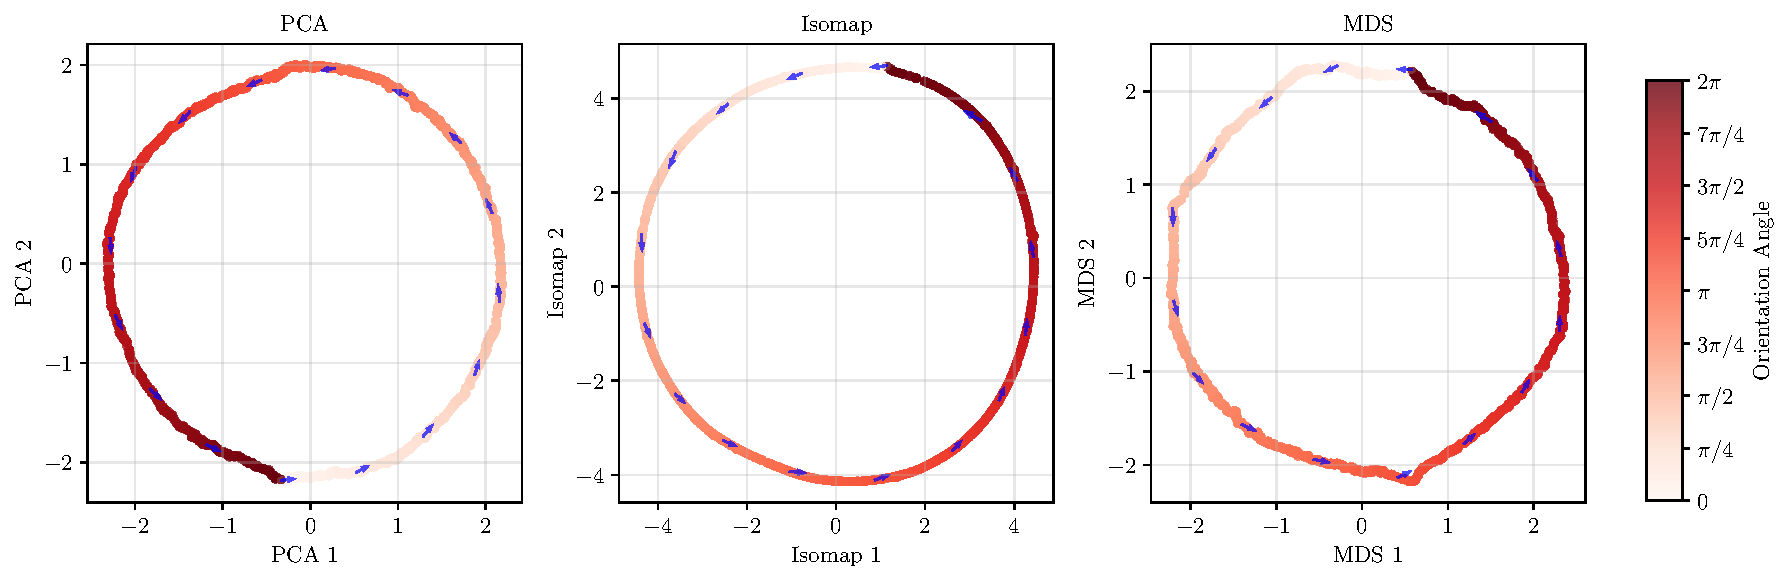
\includegraphics[width=\linewidth]{results/dim_reduction_combined.pdf}
    \captionof{figure}{Dimensionality reduction of the CNN's latent space reveals a circular manifold. Each point represents a grating stimulus, colored by orientation angle. PCA, Isomap, and MDS all recover the circular topology.}
    \vspace{0.3cm}
    \begin{itemize}
        \item Circular manifold emerged in latent space
        \item Similar orientations positioned close together
        \item Orientation space represented as continuous ring
    \end{itemize}
\end{frame}

\begin{frame}{Key Principles Demonstrated}
    \begin{itemize}
        \item \textbf{Manifold structure}: Low-dimensional manifold (circle) embedded in high-dimensional space
        \item \textbf{Topological correspondence}: Manifold topology matches task space topology
        \item \textbf{Continuous representation}: Similar stimuli mapped to nearby points
        \item \textbf{Dimensionality reduction}: High-dimensional input compressed to essential variables
    \end{itemize}
    \vspace{0.5cm}
    \begin{block}{Insight}
        Circular topology emerged naturally through backpropagation—the network discovered that a circular representation is the most efficient way to encode a periodic variable
    \end{block}
\end{frame}

\begin{frame}{Biological Neural Networks}
    % Placeholder for biological neural networks content
    \begin{itemize}
        \item Application of geometric principles to biological neural data
        \item Mouse visual cortex encodes orientation information
        \item Populations of neurons collectively form a ring-shaped manifold
        \item Manifold geometry reflects circular topology of orientation space
        \item Comparison with artificial neural network findings reveals common principles
    \end{itemize}
\end{frame}

% Conclusion section
\section{Conclusion}

\begin{frame}{Conclusion}
    \begin{itemize}
        \item Neural population geometry provides a unified framework for understanding neural computation
        \item Circular manifolds arise naturally from computational demands of the task
        \item Similar geometric structures emerge in both biological and artificial systems
        \item Comparative approach reveals common principles:
        \begin{itemize}
            \item Dimensionality
            \item Curvature
            \item Topological structure
        \end{itemize}
        \item Insights into fundamental computational strategies that transcend specific neural implementations
    \end{itemize}
\end{frame}

\begin{frame}{References}
    \begin{thebibliography}{10}
        \bibitem{demas2021high} Demas, J. et al. (2021). High-speed, cortex-wide volumetric recording of neuroactivity.
        \bibitem{yuste2015neuron} Yuste, R. (2015). From the neuron doctrine to neural networks.
        \bibitem{saxena2019towards} Saxena, S. \& Cunningham, J. P. (2019). Towards the neural population doctrine.
        \bibitem{chung2021neural} Chung, S. \& Abbott, L. F. (2021). Neural population geometry: An approach for understanding biological and artificial neural networks.
        \bibitem{chaudhuri2019intrinsic} Chaudhuri, R. et al. (2019). Intrinsic dimension of data representations in deep neural networks.
        \bibitem{beshkov2024topological} Beshkov, Y. et al. (2024). Topological analysis of neural representations.
        \bibitem{Perich2024} Perich, M. G. et al. (2024). Neural manifolds and population dynamics.
    \end{thebibliography}
\end{frame}

\end{document} 